\documentclass[11pt]{beamer}
\usepackage[UTF8,scheme=plain]{ctex}
\usepackage{listings}
\usepackage[utf8]{inputenc}
\usepackage[T1]{fontenc}
\usepackage{amsmath}
\usepackage{amsfonts}
\usepackage{amssymb}
\usepackage{graphicx}
%\usetheme{Boadilla}

\usepackage{framed} % 可以用 \begin{shaded},即背景色块
\definecolor{shadecolor}{rgb}{0.9,0.9,0.9}

\newcommand{\kong}[1][0.5]{\vspace{#1cm}}

\begin{document}
	\author{ 路毅 \hspace{0.3cm} 曲阜师范大学 }
	\date{\number\year 年 \number\month 月 \number\day 日}
	\title{数学物理方法第二章}

\begin{frame}
	\maketitle
\end{frame}

\kaishu

\begin{frame}{第二章:解析函数}
\begin{itemize}
	\item 第一节:解析函数:柯西黎曼条件
	\vspace{1cm}
	\item 第二节:解析函数与调和函数
	\vspace{1cm}
	\item 第三节:初等解析函数
\end{itemize}
\end{frame}

\begin{frame}{复变函数:可导、可微}
$\omega = f(z)$在区域$D$内有定义,若在$D$内$z$点,
\begin{equation}
f'(z) = \lim\limits_{\Delta z \rightarrow 0} \frac{\Delta \omega}{ \Delta z }
= \lim\limits_{\Delta z \rightarrow 0} \frac{ f(z + \Delta z) - f(z) }{\Delta z}
\end{equation}
存在,则称函数$f(z)$在$z$点可导。

\kong[1]

若$\omega = f(z), \Delta \omega = f(z + \Delta z) - f(z)$可写作
\begin{equation}
\Delta \omega = A(z) \Delta z + \rho(\Delta z),
\end{equation}
且 $\lim\limits_{\Delta z \rightarrow 0} \frac{ \rho(\Delta z) }{ \Delta z } = 0$。
则称$\omega = f(z)$可微,微分为
\begin{equation}
d \omega = A(z) dz.
\end{equation}

\kong[0.5]
$\omega = f(z)$可导 $\Leftrightarrow$ $\omega = f(z)$可微


\end{frame}

\begin{frame}{例题}
1. $f(z) = z^n (n=1,2,3,\cdots)$在复平面上任意点的导数,
\begin{eqnarray}
\lim\limits_{\Delta z \rightarrow 0} \frac{ (z + \Delta z)^n - z^n}{\Delta z} 
&=& \lim\limits_{\Delta z \rightarrow 0} [ nz^{n-1} +  \frac{n(n-1)}{2}z^{n-2}\Delta z + \cdots (\Delta z)^{n-1} ] 
\nonumber \\
&=& nz^{n-1}.
\end{eqnarray}

2. $f(z)=\overline{z}$在复平面上是否可微?
\begin{eqnarray}
\frac{ \overline{z+\Delta z} - \overline{z} }{ \Delta z }
= \frac{ \overline{\Delta z} }{ \Delta z },
\end{eqnarray}
上式的极限是不存在的。所以$f(z)=\overline{z}$是不可微的。
\end{frame}

\begin{frame}{和差积商的求导法则}
\begin{eqnarray}
[f(z) \pm g(z)]^\prime &=& f^\prime(z) \pm g^\prime(z), \\
\left[f(z)g(z) \right]^\prime &=& f^\prime(z) g(z) + f(z) g^\prime(z), \\
\left[ f(z)/g(z) \right]^\prime &=& \frac{f^\prime(z) g(z) - g^\prime(z) f(z)}{ [g(z)]^2 }, (g(z) \neq 0)
\end{eqnarray}
\end{frame}

\begin{frame}{柯西-黎曼条件}
\begin{equation}
\omega = f(z) = u(x,y) + i v(x,y),
\end{equation}
如果$f(z)$在$z$点可导,即
\begin{equation}
\lim\limits_{\Delta x \rightarrow 0, \Delta y \rightarrow 0}
\frac{\Delta u + i \Delta v}{ \Delta x + i \Delta y } = f^\prime (z),
\end{equation}
可导意味着:$\Delta z$为任一方向的小量,上式都得到同样的斜率$f^\prime(z)$。
\begin{itemize}
	\item $\Delta y = 0$时,得到
			\begin{equation}
			\frac{\partial u}{\partial x} + i \frac{\partial v}{\partial x} = f^\prime (z),
			\end{equation}
	\item $\Delta x = 0$时,得到
			\begin{equation}
			-i(\frac{\partial u}{\partial y} + i \frac{\partial v}{\partial y}) = f^\prime (z),
			\end{equation}
\end{itemize}
\end{frame}

\begin{frame}{柯西-黎曼条件}
所以有
\begin{equation}
\frac{\partial u}{\partial x} + i \frac{\partial v}{\partial x} = \frac{\partial v}{\partial y} - i \frac{\partial u}{\partial y}.
\end{equation}
换言之,
\begin{equation}
\left\{
\begin{aligned}
\frac{\partial u}{\partial x} &=& \frac{\partial v}{\partial y} \\
\frac{\partial v}{\partial x} &=& - \frac{\partial u}{\partial y}
\end{aligned}
\right.
\end{equation}
这就是柯西-黎曼条件(C-R条件)。我们证明了,可导$\Rightarrow$C-R条件。
\end{frame}

\begin{frame}{柯西-黎曼条件}
现有复变函数
\begin{equation}
\omega = f(z) = u(x,y) + iv(x,y),
\end{equation}
如果其中$u(x,y),v(x,y)$在$z$点可微,并且满足C-R条件,则$\omega = f(z)$在$z$点可导。

证明如下:

由C-R条件,我们设
\begin{eqnarray}
a &=& \frac{\partial u}{\partial x} |_z = \frac{\partial v}{\partial y} |_z, \\
b &=& \frac{\partial v}{\partial x} |_z = - \frac{\partial u}{\partial y} |_z,
\end{eqnarray}

因为$u(x,y),v(x,y)$在$z$点可微,所以在$z$点有
\begin{eqnarray}
\Delta u &=& a \Delta x - b \Delta y + \eta_1, \\
\Delta v &=& b \Delta x + a \Delta y + \eta_2,
\end{eqnarray}
其中
\begin{equation}
\lim\limits_{\Delta z \rightarrow 0} \frac{\eta_1}{|\Delta z|}
= \lim\limits_{\Delta z \rightarrow 0} \frac{\eta_2}{|\Delta z|} = 0,
\end{equation}
\end{frame}

\begin{frame}{柯西-黎曼条件}
所以
\begin{eqnarray}
\frac{\Delta u + i \Delta v}{\Delta x + i \Delta y}
&=& \frac{ a(\Delta x + i \Delta y) + ib(\Delta x + i\Delta y) + \eta_1 + i \eta_2}{\Delta x + i \Delta y} \\
&=& a + ib + \frac{ \eta_1 + i \eta_2}{ \Delta z }.
\end{eqnarray}
所以
\begin{equation}
\lim\limits_{\Delta z \rightarrow 0} \frac{ f(z+\Delta z) - f(z)}{\Delta z} = a + ib = f^\prime(z),
\end{equation}
这样就证明了$f(z)$可导。
\end{frame}

\begin{frame}{解析函数}
若$\omega = f(z)$在$z_0$的某个邻域内处处可微,则称$f(z)$在$z_0$点解析。

\kong[0.5]
若区域$D$内的没一点都是$f(z)$的解析点,则称$f(z)$在区域$D$内解析,或称$f(z)$是区域$D$内的解析函数(或称:全纯函数/正则函数)。

\kong[0.5]
奇点:如果$f(z)$在$z_0$点不解析,但在$z_0$的任一邻域内总有$f(z)$的解析点,则$z_0$称为$f(z)$的奇点。

\end{frame}

\begin{frame}{例题}
\begin{itemize}
	\item $f(z) = e^z = e^x(\cos y + i\sin y)$在$z$平面上是否解析?
	
	\kong[1]
	\item $f(z) = \sqrt{|xy|}$在$z=0$点是否可导?
\end{itemize}
\end{frame}

\begin{frame}{极坐标C-R条件}
设$f(z) = u(r,\theta) + iv(r,\theta)$,$z=re^{i\theta}$,若$u(r,\theta), v(r,\theta)$在$(r,\theta)$点可微,并满足极坐标下的C-R条件
\begin{equation}
\frac{\partial u}{\partial r} = \frac{1}{r}\frac{\partial v}{\partial \theta},
\frac{\partial v}{\partial r} = - \frac{1}{r}\frac{\partial u}{\partial \theta} (r>0),
\end{equation}
试证$f(z)$在$z$点是可微的,并且
\begin{equation}
f^\prime(z) = \frac{1}{e^{i\theta}}(\frac{\partial u}{\partial r} + i \frac{\partial v}{\partial r})
= \frac{1}{ire^{i\theta}}(\frac{\partial u}{\partial \theta} + i \frac{\partial v}{\partial \theta})
\end{equation}
\end{frame}

\begin{frame}{极坐标C-R条件}
证明:由于$u,v$在$(r,\theta)$点可微,有
\begin{equation}
\Delta u = \frac{\partial u}{\partial r}\Delta r + \frac{ \partial u}{ \partial \theta}\Delta \theta + \eta_1,
\end{equation}
其中$\lim\limits_{\Delta z \rightarrow 0} \frac{\eta_1}{|\Delta z|} = 0$。
另外,利用C-R条件,上式也可以写作
\begin{equation}
\Delta u = \frac{\partial u}{\partial r}\Delta r - r \frac{ \partial v}{ \partial r}\Delta \theta + \eta_1.
\end{equation}
类似地,$\Delta v$有
\begin{equation}
\Delta v = \frac{\partial v}{\partial r}\Delta r + \frac{ \partial v}{ \partial \theta}\Delta \theta + \eta_2
= \frac{\partial v}{\partial r}\Delta r + r \frac{ \partial u}{ \partial r}\Delta \theta + \eta_2.
\end{equation}
\end{frame}

\begin{frame}{极坐标C-R条件}
而$\Delta z$为
\begin{eqnarray}
\Delta z &=& (r+\Delta r)e^{i(\theta + \Delta \theta)} - re^{i\theta}
\nonumber\\
&=& (r+\Delta r)e^{i\theta} (1+i\Delta \theta + \cdots) - re^{i\theta}
\nonumber\\
&\approx& re^{i\theta}(i\Delta \theta) + \Delta r e^{i\theta} 
\nonumber\\
&=& (\Delta r + ir \Delta \theta)e^{i\theta}.
\end{eqnarray}
所以有
\begin{eqnarray}
\lim\limits_{|\Delta z| \rightarrow 0} \frac{\Delta u + i\Delta v}{\Delta z}
&=& \lim\limits_{|\Delta z| \rightarrow 0}
\frac{(\frac{\partial u}{\partial r} + i \frac{\partial v}{\partial r})(\Delta r + ir \Delta \theta) + \eta_1 + i\eta_2}{ (\Delta r + ir\Delta \theta)e^{i\theta} } 
\nonumber\\
&=& e^{-i\theta}(\frac{\partial u}{\partial r} + i\frac{\partial v}{\partial r}).
\end{eqnarray}
\end{frame}

\begin{frame}{调和函数}
若实函数$H(x,y)$在区域$D$内有二阶偏导数且
\begin{equation}
(\frac{\partial^2}{\partial x^2} + \frac{\partial^2}{\partial y^2})H = 0,
\end{equation}
则称$H(x,y)$为$D$内的调和函数。

\kong[0.5]
若$D$内两个调和函数$u,v$满足C-R条件,则称它们为共轭调和函数。

\kong[0.5]
我们注意到,如果一个解析函数$f(z)=u(x,y) + iv(x,y)$满足C-R条件,有
\begin{equation}
\left\{
\begin{aligned}
\frac{\partial u }{ \partial x} &=& \frac{\partial v}{\partial y},\\
\frac{\partial u }{ \partial y} &=& - \frac{\partial v}{\partial x}.
\end{aligned}
\right.
\Rightarrow
\left\{
\begin{aligned}
\frac{\partial^2 u}{ \partial x^2} + \frac{\partial^2 u}{\partial y^2} &=& 0,\\
\frac{\partial^2 v}{ \partial x^2} + \frac{\partial^2 v}{\partial y^2} &=& 0.\\
\end{aligned}
\right.
\end{equation}
也就是说,\color{blue}$f(z)=u+iv$在$D$内解析$\Leftrightarrow$ $u,v$为$D$内的共轭调和函数。
\end{frame}

\begin{frame}{调和函数}
若$u$已知,$v$未知,但是$u,v$为共轭调和函数,则有
\begin{equation}
dv = v_x dx + v_y dy = - u_y dx + u_x dy,
\end{equation}
因为$u,v$是共轭调和函数,所以有
\begin{equation}
\frac{\partial}{\partial y}(- u_y) = \frac{\partial}{\partial x} (u_x),
\end{equation}
所以上面写的$dv$是全微分,即
\begin{equation}
v(z) = \oint^z_{z_0}(-u_y dx + u_x dy),
\end{equation}
这里积分路径是$D$内任意曲线。

\kong[0.5]
换言之,用$u$可以求出它的共轭调和函数$v$。若$v$已知,也可以类似地求出$u$。
\end{frame}

\begin{frame}{共轭调和函数的几何意义}
函数$u$在xy平面上的梯度为
\begin{equation}
\vec{\nabla}u = (u_x, u_y) = (v_y, - v_x),
\end{equation}
函数$v$在xy平面上的梯度为$\vec{\nabla} v = (v_x, v_y)$,所以有
\begin{equation}
\vec{\nabla}u \cdot \vec{\nabla} v = (v_y, -v_x)(v_x, v_y) = 0.
\end{equation}
这意味着,函数$u,v$的梯度处处垂直,相应地,它们的“等高线”也处处垂直。
\end{frame}

\begin{frame}{共轭调和函数}
\begin{figure}
	\centering
	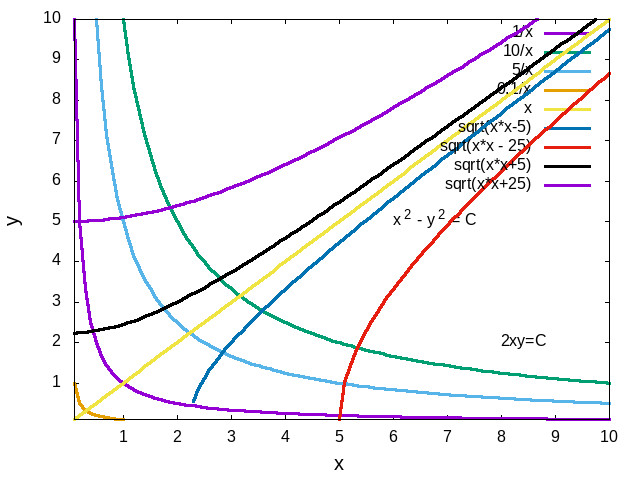
\includegraphics[width=0.6\linewidth, height=0.6\linewidth]{chap2_01.jpeg}
	\caption{共轭调和函数“等高线”处处垂直}
	\label{fig:chap201}
\end{figure}
\end{frame}

\begin{frame}{初等解析函数,整数幂函数}
我们证明以下初等函数是解析函数
\begin{equation}
z^n, e^z, \sin z, \cos z, \sinh z, \cosh z, z^{1/n}, \ln z, z^a, \arcsin z
\end{equation}

1. 幂函数 $\omega = z^n, n=1,2,3,\cdots$,前面已经证明过,它在整个复平面上解析,
\begin{equation}
\lim\limits_{\Delta z \rightarrow 0} \frac{ (z+\Delta z)^n - z^n}{\Delta z} = n z^{n-1}.
\end{equation}
容易证明:
\begin{eqnarray}
\omega = P(z) = a_0 z^n + a_1 z^{n-1} + \cdots + a_n, (a \neq 0),
\end{eqnarray}
在复平面上解析;
\begin{equation}
\omega = \frac{P(z)}{Q(z)} = \frac{a_0 z^n + \cdots + a_n}{b_0 z^n + \cdots b_n}, (a_0, b_0 \neq 0)
\end{equation}
在复平面上除$Q(z)$的零点外解析。
\end{frame}

\begin{frame}{初等解析函数:$e$指数函数}
$e$指数函数定义为:
\begin{equation}
\omega = e^z = e^{x+iy} = e^x(\cos y + i\sin y),
\end{equation}
容易证明:
\begin{eqnarray}
|e^z| &=& |e^x e^{iy}| = e^x >0, \\
e^{z_1} e^{z_2} &=& e^{z_1 + z_2}, \\
\frac{d\omega}{dz} &=& \lim\limits_{\Delta z \rightarrow 0}
\frac{ e^{z+\Delta z} - e^z}{\Delta z} = \lim\limits_{\Delta \rightarrow 0} \frac{ e^z(e^{\Delta z} -1) }{ \Delta z}
= e^z, \\
e^{z + 2\pi k i} &=& e^z.
\end{eqnarray}
\end{frame}

\begin{frame}{三角函数、双曲函数}
复数域上的三角函数定义为
\begin{eqnarray}
\cos z &=& \frac{e^{iz} + e^{-iz}}{2}, \\
\sin z &=& \frac{e^{iz} - e^{-iz}}{2i},
\end{eqnarray}
因为$e^{iz}, e^{-iz}$是解析的,所以三角函数是解析的。

\kong[0.5]
双曲函数定义为
\begin{eqnarray}
\sinh z &=& \frac{e^z - e^{-z}}{2}, \\
\cosh z &=& \frac{e^z + e^{-z}}{2}.
\end{eqnarray}
\end{frame}

\begin{frame}{多值函数:根式函数}
\begin{equation}
\omega = z^{1/n},
\end{equation}
记$\omega = \rho e^{i\varphi}, z = re^{i\theta}$,可以推出
\begin{eqnarray}
\rho &=& r^{1/n}, \\
\varphi &=& \frac{\theta}{n} + k \frac{2\pi}{n}, k \in Z,
\end{eqnarray}
即
\begin{equation}
\omega = r^{1/n} e^{i (\frac{\theta}{n} + k \frac{2\pi}{n}) },
k = 0, 1, \cdots, n-1
\end{equation}
$k$的$n$个取值定义了$\omega = f(z)$的$n$个{\color{blue}单值分支}
\begin{equation}
\omega_k = (z^{1/n})_k = r^{1/n} e^{i\frac{\theta + 2k\pi}{n}}, k = 0,1,\cdots,n-1
\end{equation}
\end{frame}

\begin{frame}{根式函数:每个单值分支可导}
\begin{equation}
\omega_k = (z^{1/n})_k = r^{1/n} e^{i\frac{\theta + 2k\pi}{n}}, k = 0,1,\cdots,n-1
\end{equation}
所以$\omega_k$的实部、虚部为
\begin{eqnarray}
u &=& r^{1/n} \cos \frac{\theta + 2k\pi}{n}, \\
v &=& r^{1/n} \sin \frac{\theta + 2k\pi}{n},
\end{eqnarray}
这两个函数都可微,并且有
\begin{eqnarray}
\frac{\partial u}{\partial r} &=& \frac{1}{n} r^{1/n -1} \cos \frac{ \theta + 2k\pi}{n}, \\
\frac{\partial u}{\partial \theta} &=& - \frac{1}{n} r^{1/n} \sin \frac{ \theta + 2k\pi}{n}, \\
\frac{\partial v}{\partial r} &=& \frac{1}{n} r^{1/n -1} \sin \frac{ \theta + 2k\pi}{n}, \\
\frac{\partial v}{\partial \theta} &=& \frac{1}{n} r^{1/n} \cos \frac{ \theta + 2k\pi}{n}, 
\end{eqnarray}
\end{frame}

\begin{frame}{根式函数:每个单值分支可导}
可得
\begin{eqnarray}
\frac{\partial u}{\partial r} &=& \frac{1}{r} \frac{\partial v}{\partial \theta}, \\
\frac{\partial v}{\partial r} &=& - \frac{1}{r} \frac{\partial u}{\partial \theta}, \\
\end{eqnarray}
所以$z^{1/n}$的每个单值分支$\omega_k$都是解析函数,其导数为
\begin{equation}
\frac{d \omega_k}{d z} = e^{-i\theta}(\frac{\partial u}{\partial r} + i \frac{\partial v}{\partial r}) = \frac{1}{n}z^{1/n -1 },
\end{equation}
与整数幂函数求导公式完全一致。
\end{frame}

\begin{frame}{支点、支割线}
若取$z^{1/n}$的第一支
\begin{equation}
\omega_0 = r^{1/n} e^{i \theta/n},
\end{equation}
让$z$沿原点绕一圈,$\omega_0$将变为$r^{1/n}e^{i \frac{\theta + 2\pi}{n} } = \omega_1$。

\kong[0.5]
支点:$z$绕支点一周,函数$\omega=f(z)$将从一个分支变为另一个分支。

\kong[0.5]
无穷远点也是$z^{1/n}$的一个支点。

\end{frame}

\begin{frame}{支割线}
从支点$z=0$到$z=\infty$引一条射线,割开$z$平面,如
\begin{equation}
0 \leq arg z < 2\pi,
\end{equation}
则不会有闭合曲线绕过原点,即不会从一支连续变为另一支。
\end{frame}

\begin{frame}{(以$e$为底的)对数函数}
(以$e$为底的)对数函数是$e$指数的反函数
\begin{equation}
z = e^\omega \Rightarrow \omega = Ln z,
\end{equation}
可得
\begin{equation}
Ln z = \ln r + i(\theta + 2k\pi), k = 0, \pm 1, \pm 2, \cdots
\end{equation}
主值支:
\begin{equation}
\ln z = \ln r + i arg z,
\end{equation}
其中$arg z$为$z$的辐角主值,区间可定义为$(-\pi, \pi]$或者$[0,2\pi)$。
不同分支的值域构成复平面上的不同区域
\begin{eqnarray}
&& -\pi < v \leq \pi, \\
&& \pi < v \leq 3 \pi, \\
&& \cdots
\end{eqnarray}
$z=0, \infty$是$Ln z$的支点,
\begin{equation}
(\ln z)_k = \ln r + i(\theta + 2k\pi), k=0, \pm 1, \pm 2, \cdots
\end{equation}
\end{frame}

\begin{frame}{(以e为底的)对数函数}
容易证明:
\begin{eqnarray}
\frac{d}{dz}(\ln z)_k &=& \frac{1}{z}, k=0, \pm 1, \pm 2, \cdots \\
Ln (z_1 z_2) &=& Ln z_1 + Ln z_2, \\
Ln (z_1 / z_2) &=& Ln z_1 - Ln z_2,
\end{eqnarray}
\end{frame}

\begin{frame}{一般幂函数}
\begin{equation}
z^a = e^{a Ln z} = \omega_0 e^{i 2k\pi a}, k=0, \pm 1, \pm 2, \cdots
\end{equation}
其中$\omega_0 = e^{a \ln z}$。

\kong[0.5]
若$a$为整数$n$,则$e^{2k\pi i a} = 1, z^a = \omega_0$是一个单值函数。

\kong[0.5]
若$a$为有理数$q/p$,则
\begin{equation}
e^{2k\pi i a} = e^{2k\pi i q/p}, k=0,1,\cdots,p-1
\end{equation}
所以有
\begin{equation}
z^{q/p} = \omega_0 e^{2k\pi i q/p}, k=0,1,\cdots,p-1
\end{equation}
有$p$个分支。

\kong[0.5]
若$a$为无理数,则有无穷多个分支。

一般幂函数的导数为
\begin{equation}
\frac{d}{dz}(z^a)_k = \frac{d}{dz} e^{a(\ln z)_k} = a z^{a-1}.
\end{equation}

\end{frame}

\begin{frame}{一般指数函数}

\begin{equation}
\omega = a^z = e^{z Ln a},
\end{equation}
有无穷多分支。

\kong[0.5]
$a=e$时,$\omega = e^z$是特殊的单值函数。
\end{frame}

\begin{frame}{反三角函数}
若有
\begin{equation}
z = \sin \omega = \frac{ e^{i\omega} - e^{-i\omega}}{2i},
\end{equation}
得到
\begin{eqnarray}
&& (e^{i\omega})^2 - 2i z e^{i\omega} -1 = 0, \\
\omega &=& \arcsin z = \frac{1}{i} Ln (iz + \sqrt{1-z^2} ) \\
       &=& \frac{\pi}{2} + \frac{1}{i} Ln (z + \sqrt{z^2 -1}),
\end{eqnarray}
类似地,
\begin{equation}
\arccos z = \frac{1}{i} Ln (z + \sqrt{z^2 -1} ).
\end{equation}
它们都是多值函数。
\end{frame}

\begin{frame}{作业}

\kong[0.5]
课堂讲解:8, 13, 19

\kong[0.5]
课下练习:1, 2, 5, 9, 14, 15
\end{frame}

\end{document}